\chapter{Predicting the Future}

\section{Idea}

The first policy we look at is formerly called Multi-Level Feedback Queue or MLFQ short. The create Fernando J. Corbató recieved a Turning Award for it in 1990. 
As the title already says, this policy tries to predict the future behaviour of the processes based on the past.
A job can be generally act in two ways.
Either it is a resources intensive crunching problem (think about exporting a video or compiling code) or it is a program, which needs quick response time (think about your text editor).
In reality most jobs jump between these two states.
We usually want to give the response based processes priority, because that is what the user interacts with and it is here that he primarily feels a delay.

The policy is based on multiple queues, which have each different priorities.
Each process gets assigned to a queue. There are however not set in stone
Based on the reasons above we want to assume that a new process is responsive, because in the worst case scenario, we need to just demote the non-responsive ones.
If however a process turns out to be interactive, than the user does not feel any lag. 
Each process can run a certain amount of time (also called allotment time) before it is deemed as unworthy of the current priority.
If the allotment is used up the process get demoted into a queue below.

\begin{figure}[h]
    \centering
    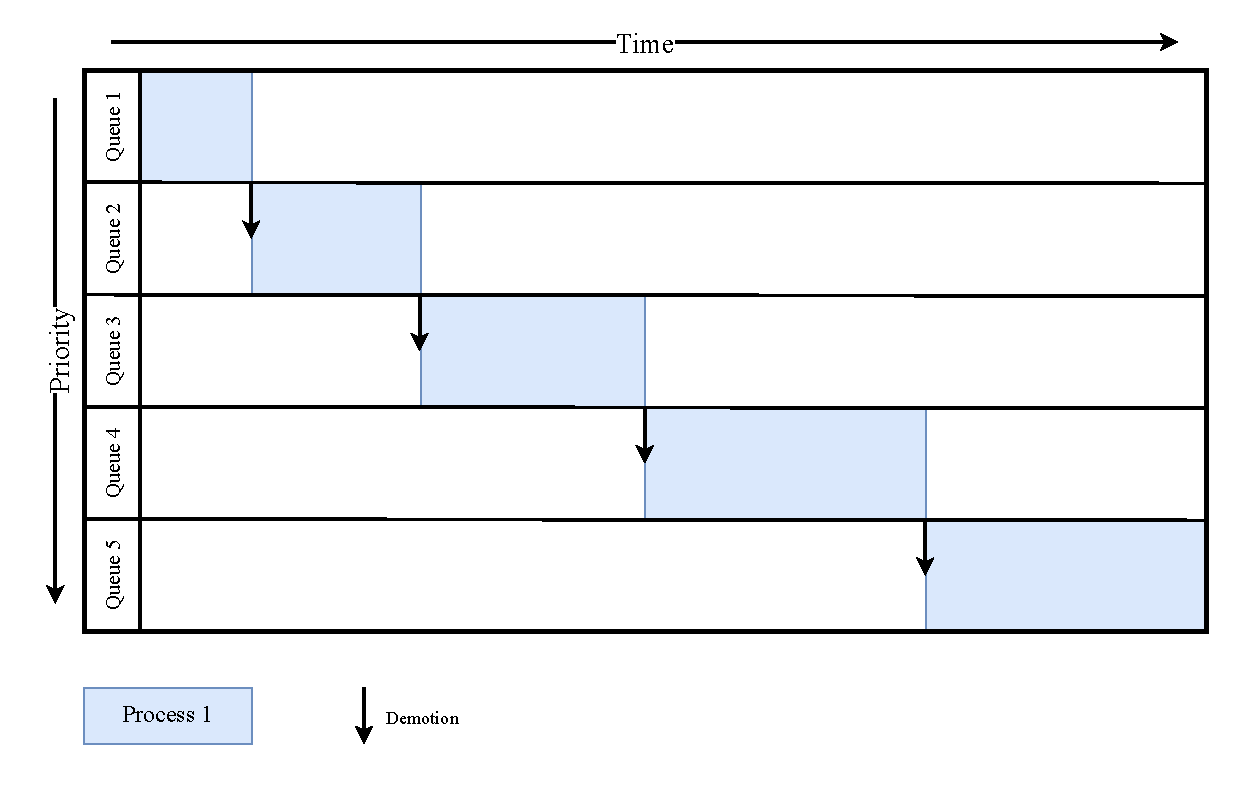
\includegraphics[width=0.7\textwidth]{Assets/MLFQ-Example-1.pdf}
    \caption{Simple working of MLFQ}
    \label{fig:mlfq-example-1}
\end{figure}


As you can see in figure \ref{fig:mlfq-example-1} the process one gets demoted after a while.
Also the lower the queue is, the higher the allotment time. 
This is because we hope that all of the responsive focused finish before demoting.
Once these are filtered out we have only resource heavy tasks left.
These require more time anyways, so the allotment time is stretched out.

\section{Multiple Processes}

What happens if we introduce another process?
Well, it depends on the priorities. 
Higher priority recieves the CPU time.
If they are on the same queue, than they run using Round Robin, see section \ref{sec:rr}.


\begin{figure}[h]
    \centering
    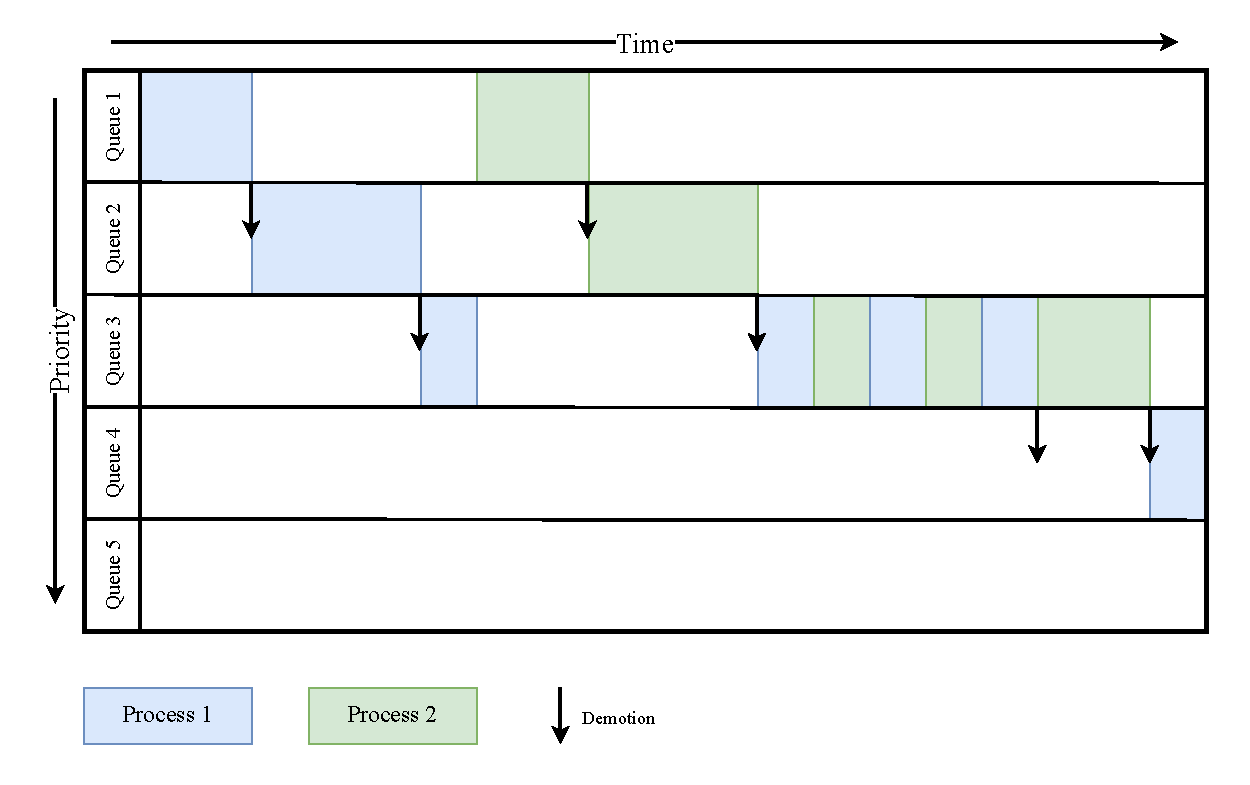
\includegraphics[width=0.7\textwidth]{Assets/MLFQ-Example-2.pdf}
    \caption{Running multiple processes in MLFQ}
    \label{fig:mlfq-example-2}
\end{figure}

As you can see in figure \ref{fig:mlfq-example-2} once process two is introduced process one is temporarily starved. The problem is solved once they land on the same queue.
There they run alternately.
Still the more tasks we introduce the more prevalent the starving issue gets.

\begin{figure}[h]
    \centering
    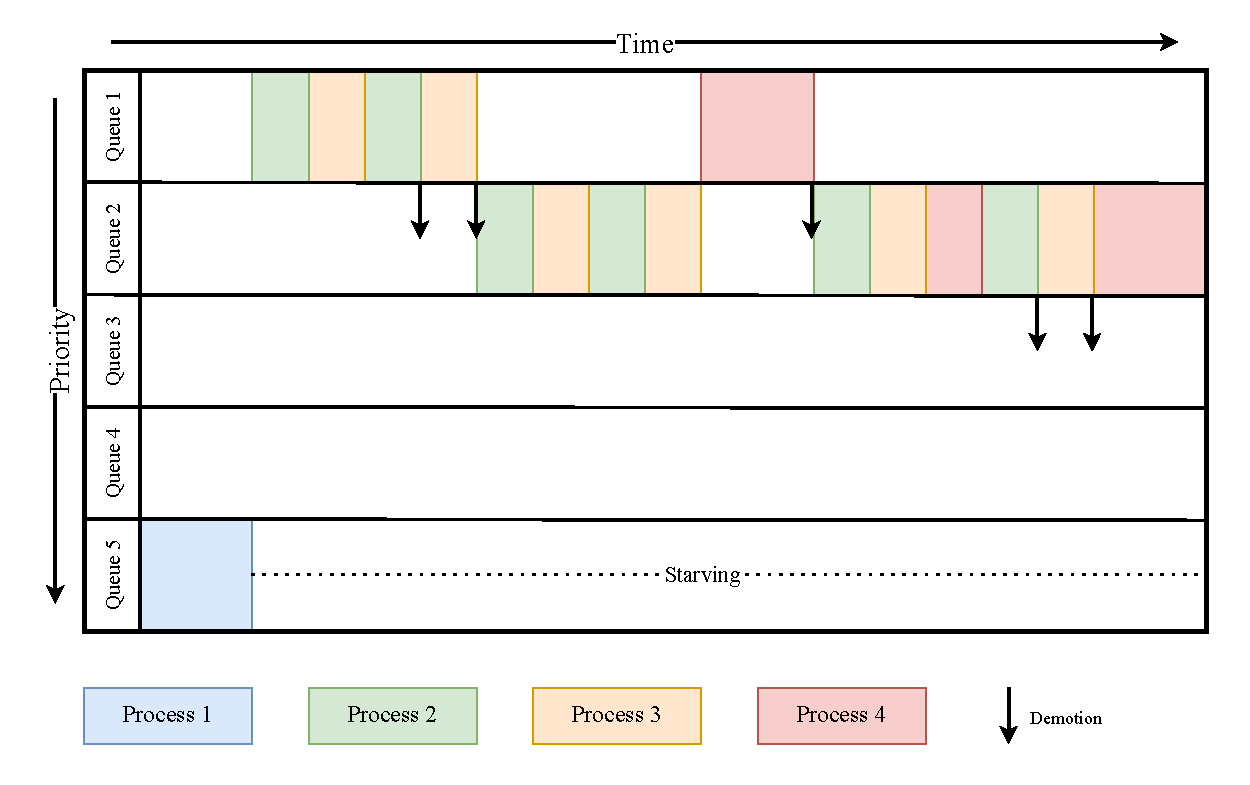
\includegraphics[width=0.7\textwidth]{Assets/MLFQ-Example-3.pdf}
    \caption{Starving Processes in MLFQ}
    \label{fig:mlfq-example-3}
\end{figure}

\section{Solving the Starving Problem}

Solving starvation is actually easy.
All we have to make sure that once in a while everybody gets their deserved CPU time.
To do that we introduce a priority boost. All it does is just put every process into priority one every so often.

\begin{figure}[h]
    \centering
    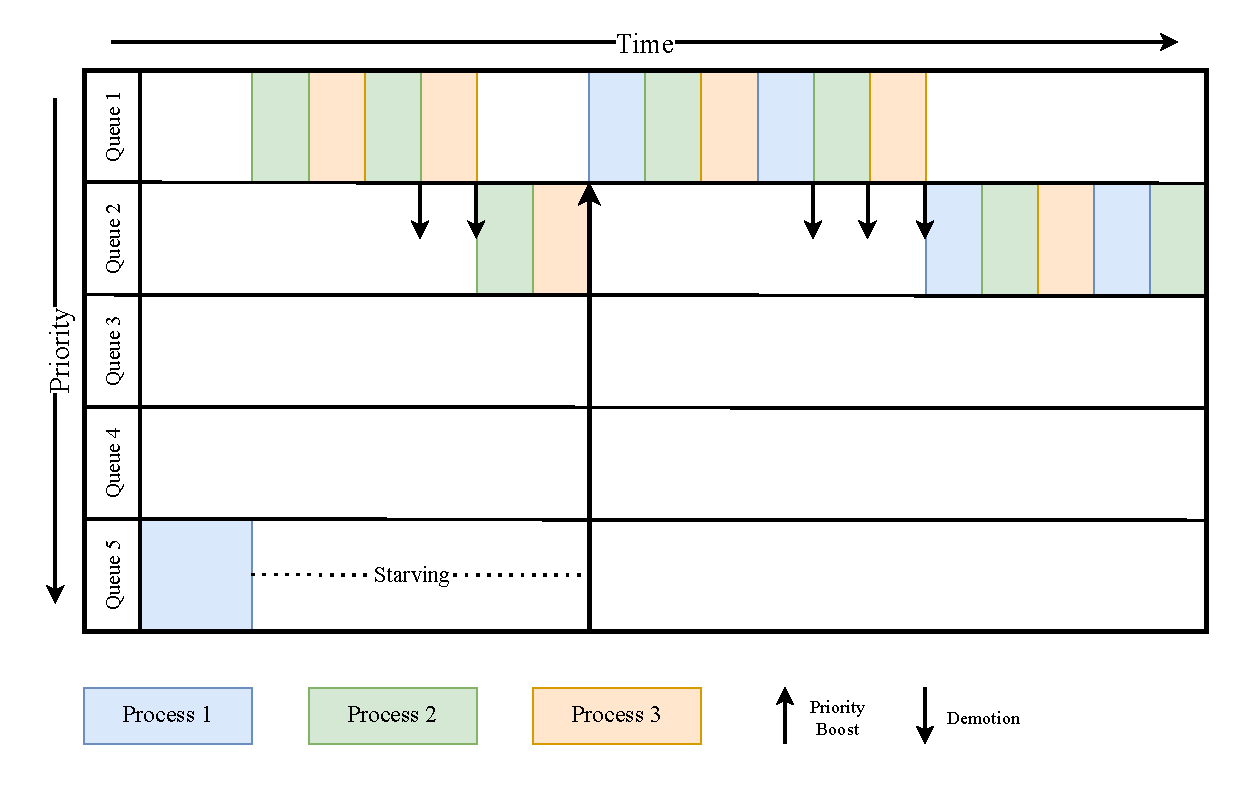
\includegraphics[width=0.7\textwidth]{Assets/MLFQ-Example-4.pdf}
    \caption{Solving Starvation in MLFQ}
    \label{fig:mlfq-example-4}
\end{figure}

\section{Wrapping Up}

This chapter showed us, how one could approach a scheduling policy that works without needing to know the burst time.
In the end we still end up with many variable like the allotment time per queue, the amount of queues, the quanta for the Round Robin and others.
If used in a real system the best approach would be to set some sensible defaults and let the administrator to adjust the parameters when needed.

\chapter{Using Lottery to Schedule Processes}